
% ***************************************************
% Example of an internal chapter
% ***************************************************
%This is an internal chapter of the thesis.
%If you have a long title, you can supply an abbreviated version to print in the Table of Contents using the optional argument to the \chapter command.
\chapter[Results]{Results and Discussion}
\label{Chap:label}	%CREATE YOUR OWN LABEL.
\pagestyle{headings}

This chapter aims to demonstrate the practicality and efficacy of the designed hardware. Performance metrics such as latency, resource utilisation, timing, and power consumption are analysed to gauge the design's effectiveness. The design is also tested with a small sample of real life packets of different properties to ensure the packet filter can correctly block unwanted packets. Preexisting solutions are then compared with the design, providing insight into the design's relative strength and weaknesses in areas of latency, power and thermal performance.



\section{Latency Performance}

Reducing the latency of hardware packet filtering in embedded systems is one of the key objectives of this thesis. As such, verification of the latency added due to the filtering is essential.

\subsection{Theoretical analysis}
The design employs a 200-stage shift register to temporarily store the incoming packet with each stage being 2bits wide. Given a clock frequency of 50Mhz, the added latency can be calculated to be $200 \times \frac{1}{50\times 10^6} = 4 \times 10^{-6} = 4\mu s$.

\subsection{Measured analysis}


The packet classifier's performance was measured with an Agilent MSO6054A MSO due to its high sampling rate of 4GSa/s. A PMOD pin was connected to output of an xor operation between the carrier sense line (crs\_dv) from the PHY and the crs\_dv post packet filtering. 

This process allowed the added latency to be measured characterised by the time between the rising and falling edge of either pulse as shown in figure \ref{fig:pf_added_latency}. The measured output can be seen to match the theoretical calculation of $4\mu s$.


\begin{figure}[h!]
    \centering
    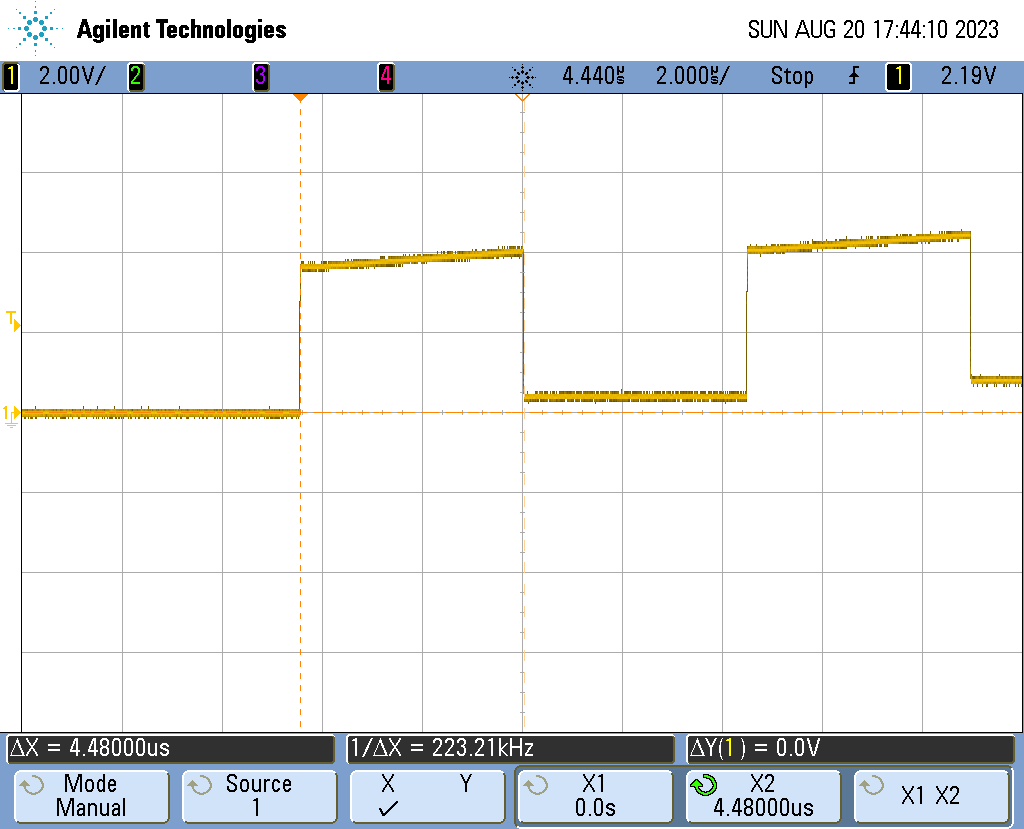
\includegraphics[width=0.75\textwidth]{Images/scope_4.png}
    \caption[Added latency by packet filter waveform]{Added latency by packet filter waveform.}
    \label{fig:pf_added_latency}
\end{figure}


The two distinct pulses are a result of the phase shift between the PHY crs\_dv and the delayed crs\_dv line. Additionally, the distance between the two pulses indicates the size of the packet. 


\subsection{Improvements}
A potential improvement on the design could be to integrate the packet classifier with the Ethernet MAC. This could reduce the added latency to zero by removing the need to store the packet in the additional shift register. The approach would involve storing the incoming packet and if the packet is later deemed to be blocked, the controlling FSM could be reset to ignore the packet. 











\section{Utilisation}

Resource utilisation is an integral part in validating the feasibility of implementing the design on a particular FPGA or microchip. This section details the post synthesis resource utilisation of the design on the Nexys A7-100T FPGA using Xilinx Vivado 2022.2. Namely, the NEORV32, Ethernet hardware and packet filter are analysed.


The resource breakdown referred to in this section can be found in figure \ref{fig:resource_util} while a more detailed breakdown of the resource utilisation including the primitives can be found in appendix \ref{app:res_usage}. 

\begin{figure}[h]
    \centering
    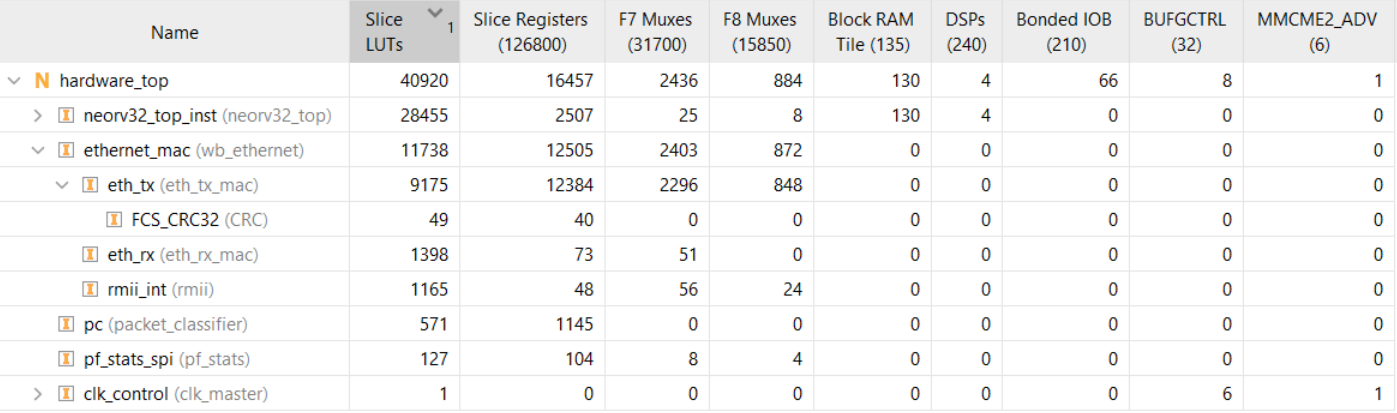
\includegraphics[width=1\textwidth]{Images/FPGAUtilisationResources.png}
    \caption[Summary of the resource utilisation on XC7A100T FPGA]{Summary of the resource utilisation on XC7A100T FPGA.}
    \label{fig:resource_util}
\end{figure}

 
The design as a whole uses a total of 64.5\% of the available slice LUTs, 12.9\% of the available flip flops and 96.3\% of the available BRAM.




\subsection{NEORV32 processor}

significant LUT usage was attributed to the 32-bit wide wishbone interface. Considerable LUT consumption relates to frame buffers used in Ethernet hardware, elucidated further in subsection \ref{sec:eth_hardware_util}.


The NEORV32 SoC consumed the majority (69.5\%, or 28455), of the slice LUTs in the design. While many interfaces were enabled such as SPI, UART, GPIO, external interupts (XIRQ) and the true random number generator, a considerable amount of the LUTs were consumed by the 32bit wide wishbone interface. More specifically, 25992 slice LUTs, or 91.3\% of the NEORV32 usage. 

The large LUT utilisation relates to the frame buffers used in the Ethernet hardware, elucidated further in section \ref{sec:eth_hardware_util}. 

DSP48 blocks were also used by the SoC to handle the multiply operations to free up LUTs. 

The instruction memory (IMEM) and data memory (DMEM) sizes were configured to optimise the remaining BRAM blocks for increasing flexibility in firmware. Specifically, IMEM was allocated 256KB while the DMEM (acting as RAM) amounting to 168KB. 





\subsection{Ethernet hardware}
\label{sec:eth_hardware_util}


Comparatively, the Ethernet hardware accounted for 11738 slice LUTs and 12505 slice registers, most of which is consumed by the transmit logic (78\% LUT and 99\% registers). The considerable LUT utilisation in the transmit logic and NEORV32 Wishbone interface is due to the manner in which the frame buffer is written to. The complex operations such as address validation and array modification for writing to the frame buffer can be seen in listing \ref{lst:code_snippet}. Notably, the address validation specifically implements a 32bit wide comparator and the need to write/modify to the frame buffer array causes large LUT utilisation.

\begin{lstlisting}[style=vhdl, caption={Code for writing to the frame buffer}, label=lst:code_snippet]
if wb_i_addr >= x"13371004" and wb_i_addr <= x"13376410" then         
    -- Subtract 4100 from the address to get the virtual address
    virtAddr := to_integer((unsigned(wb_i_addr(15 downto 0)) - 4100));
    FRAME_BUFFER(8 + virtAddr) := wb_i_dat(31 downto 24);
    FRAME_BUFFER(9 + virtAddr) := wb_i_dat(23 downto 16);
    FRAME_BUFFER(10 + virtAddr) := wb_i_dat(15 downto 8);
    FRAME_BUFFER(11 + virtAddr) := wb_i_dat(7 downto 0);
end if;
\end{lstlisting}

This design choice also influenced the critical path delay as detailed further in section \ref{sec:timing_summary}. Optimisations to this area would be imperative to drastically reduce the resource consumption and improve the critical path delay.

By contrast, the receive logic consumed far less resources of 12\% of the Ethernet MAC's LUTs and only 1\% of the registers. This is attributed to the simpler design which stores the incoming packets with the correct endianness in the frame buffer before subsequently triggering an interrupt upon the packet's arrival. 

The rmii\_init logic acts as the glue logic between the PHY and the MAC. It facilitates the clock and bus domain crossings between the 8bit wide 80Mhz MAC and the 2bit wide 50Mhz RMII PHY. 



\subsection{Packet filter}

The packet classifier consumed a total of 571 slice LUTs and 1145 slice registers, suggesting a potential to increase the number of rules. Though, the fan-in and fan-out will likely need to be considered due to the nature of the implementation. The synthesiser's decision to use registers over BRAM for rule storage is likely due to the rules being small in size and that the BRAM blocks are better used elsewhere.

Alternatively, the minimal resource utilisation indicates that the design is suitable for implementation on smaller FPGAs or ASIC designs and will have negligible impact on the overall silicon area.





\section{Timing Summary}
\label{sec:timing_summary}


Timing analysis of the design provides insight into the critical path delay and the maximum frequency of the design. Basic results are presented in this section and are primarily around the Wishbone interface due to its role in the critical path. Importantly, the Wishbone interface operates at the same clock frequency as the NEORV32 processor which directly impacts the speed of the CPU for software based operations.

Initially, a single 50Mhz clock sourced from the onboard MMCM was used. A post-synthesis analysis indicated a positive slack in the design, allowing for the clock frequency to be updated to 80Mhz. This was done to increase the performance of the CPU so that it could process network packets faster in software.

After resynthesising, a worst negative slack for setup time of -2.634ns was reported with a total of 82 endpoints failing the constraints. Additionally, a worst hold slack of -0.021ns was reported. The identified critical path originates from the Wishbone interface to the BRAM block within the Ethernet hardware, shown in figure \ref{fig:crit_path}. Due to the NEORV32's implementation of the Wishbone bus, the critical path cannot be easily improved and is the leading limitation in the speed of the design. 


\begin{figure}[h]
    \centering
    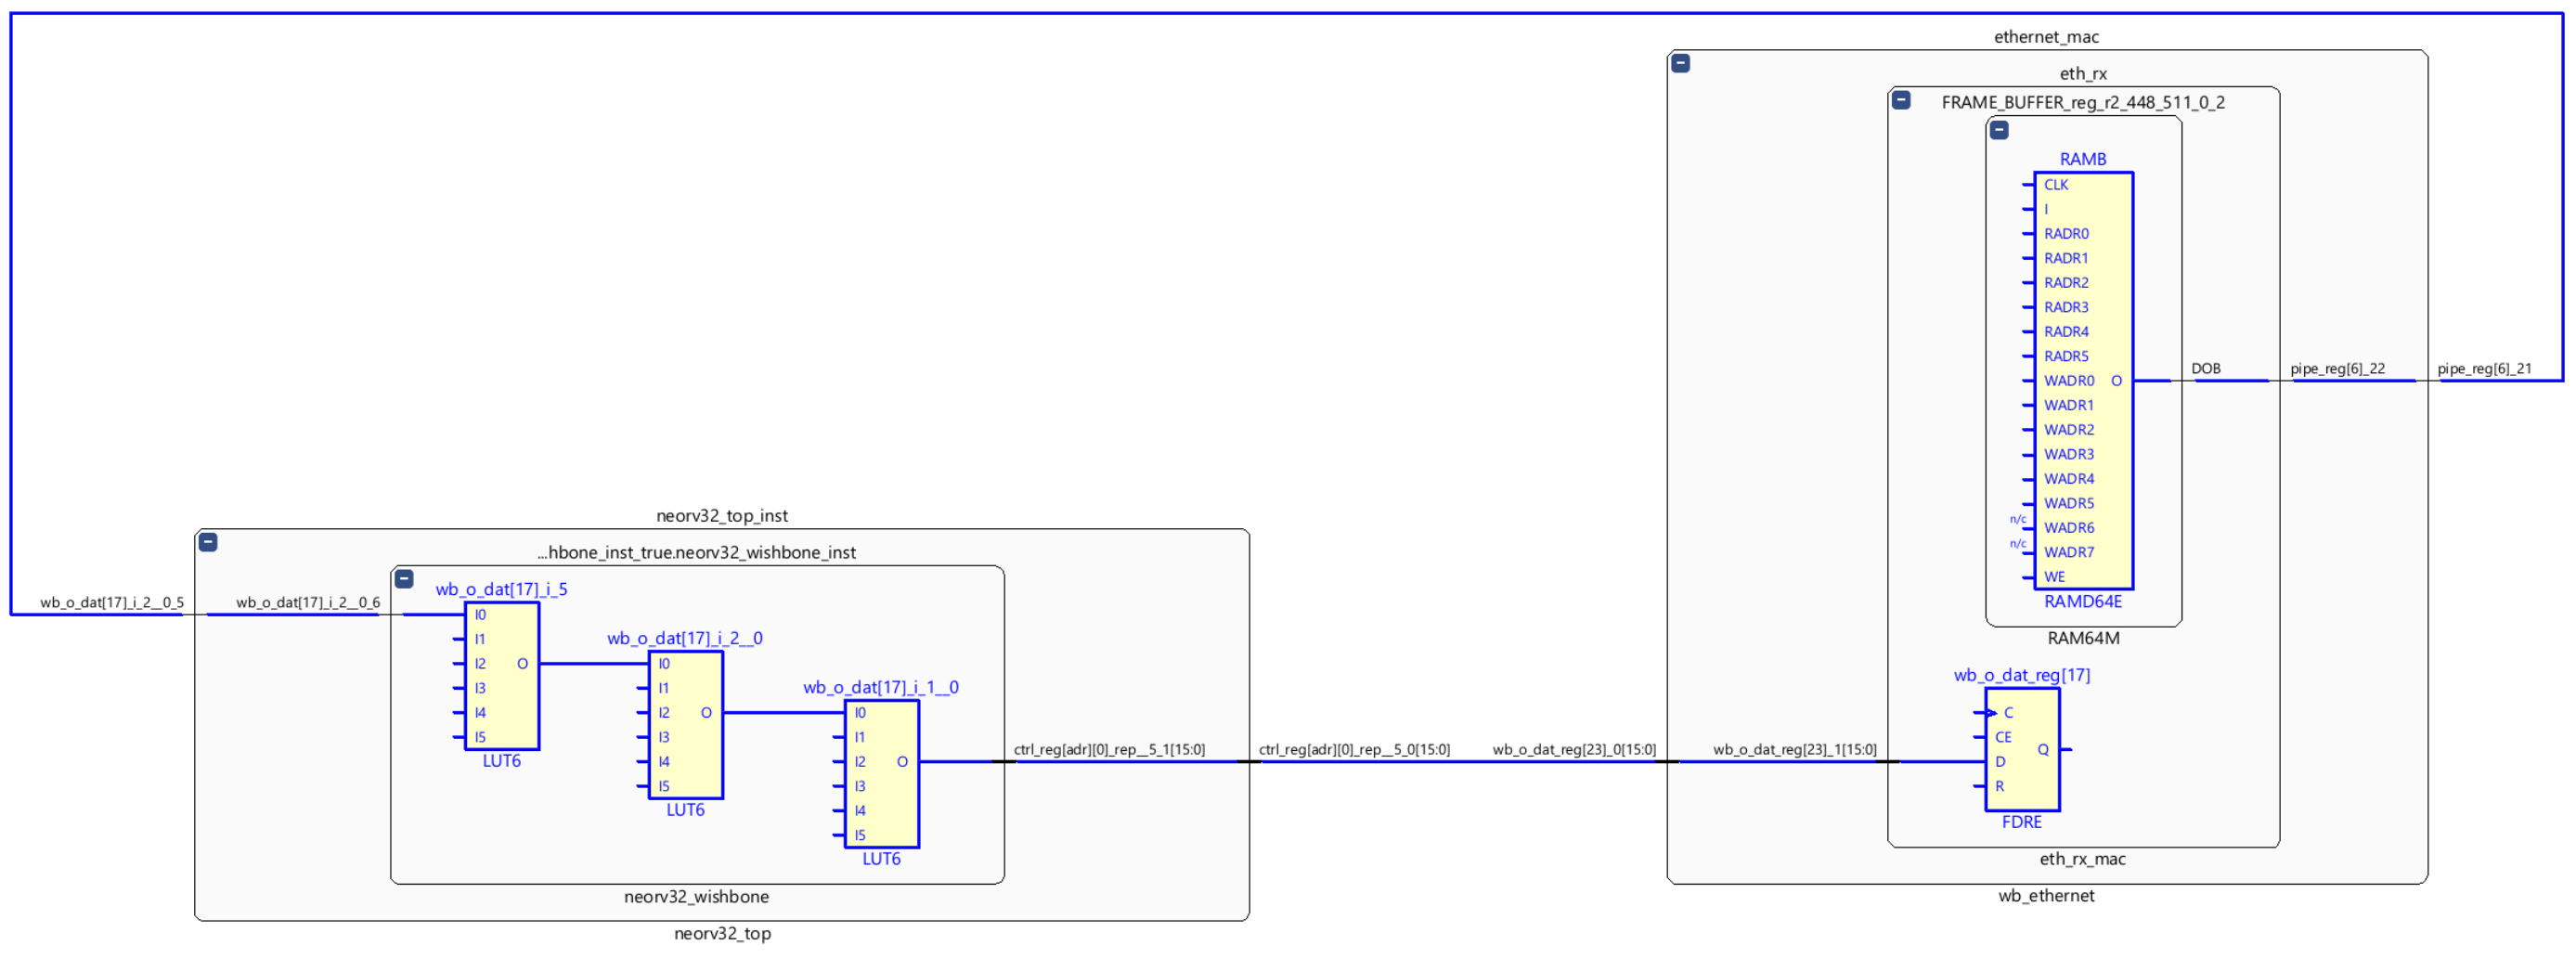
\includegraphics[width=1\textwidth]{Images/critical_path_delay_schematic.png}
    \caption[Critical path in SoC design]{Critical path in SoC design.}
    \label{fig:crit_path}
\end{figure}


While in practice these timing constraints do not crucially impact the design's operation, caution is advised in future adaptations or usage. Other paths were also encroaching on a slack of zero and hence the design was limited to 80Mhz. Testing at 90Mhz was conducted, however, the design was found to be unstable and had a large increase in the number of failing endpoints.

More accurate timing constraints would need to be set to acquire the absolute maximum frequency of the design. Though, this was outside the scope of this thesis. 





















\section{Filtering performance}

Blocking unwanted packets is imperative to a firewall's operation with any packets bypassing the filter rendering it useless. Testing all possible permutations of bits going through the firewall is infeasible due to the sheer number of packets needed, which is on the order of $2^{104}$. For example, a complete testing suite for all source IP addresses alone would require $2^32$ (about 4.3 billion) packets to be sent to the device. Therefore, a small sample of packets, shown in table \ref{tab:firewall_testing_config}, were tested to ensure the filter is working as intended. 


\subsection{Test setup}

Four hosts distributed across two networks were used to test the device as depicted in the network diagram in figure \ref{fig:network_layout_test}. The network consisted of three Raspberry Pi 4s and an x86 based Ubuntu machine. The specifics characteristics of these devices are irrelevant to this thesis, given that they all adhere to the TCP/IP standards. More specifically they were chosen due to their capability to run python scripts and are accessibility over Ethernet. A common script\footnote[1]{The python \textit{test} script can be found at https://github.com/matty0005/thesis-tools} was used on all devices to test each of the services available on different ports and protocols. 



\begin{figure}[h]
    \centering
    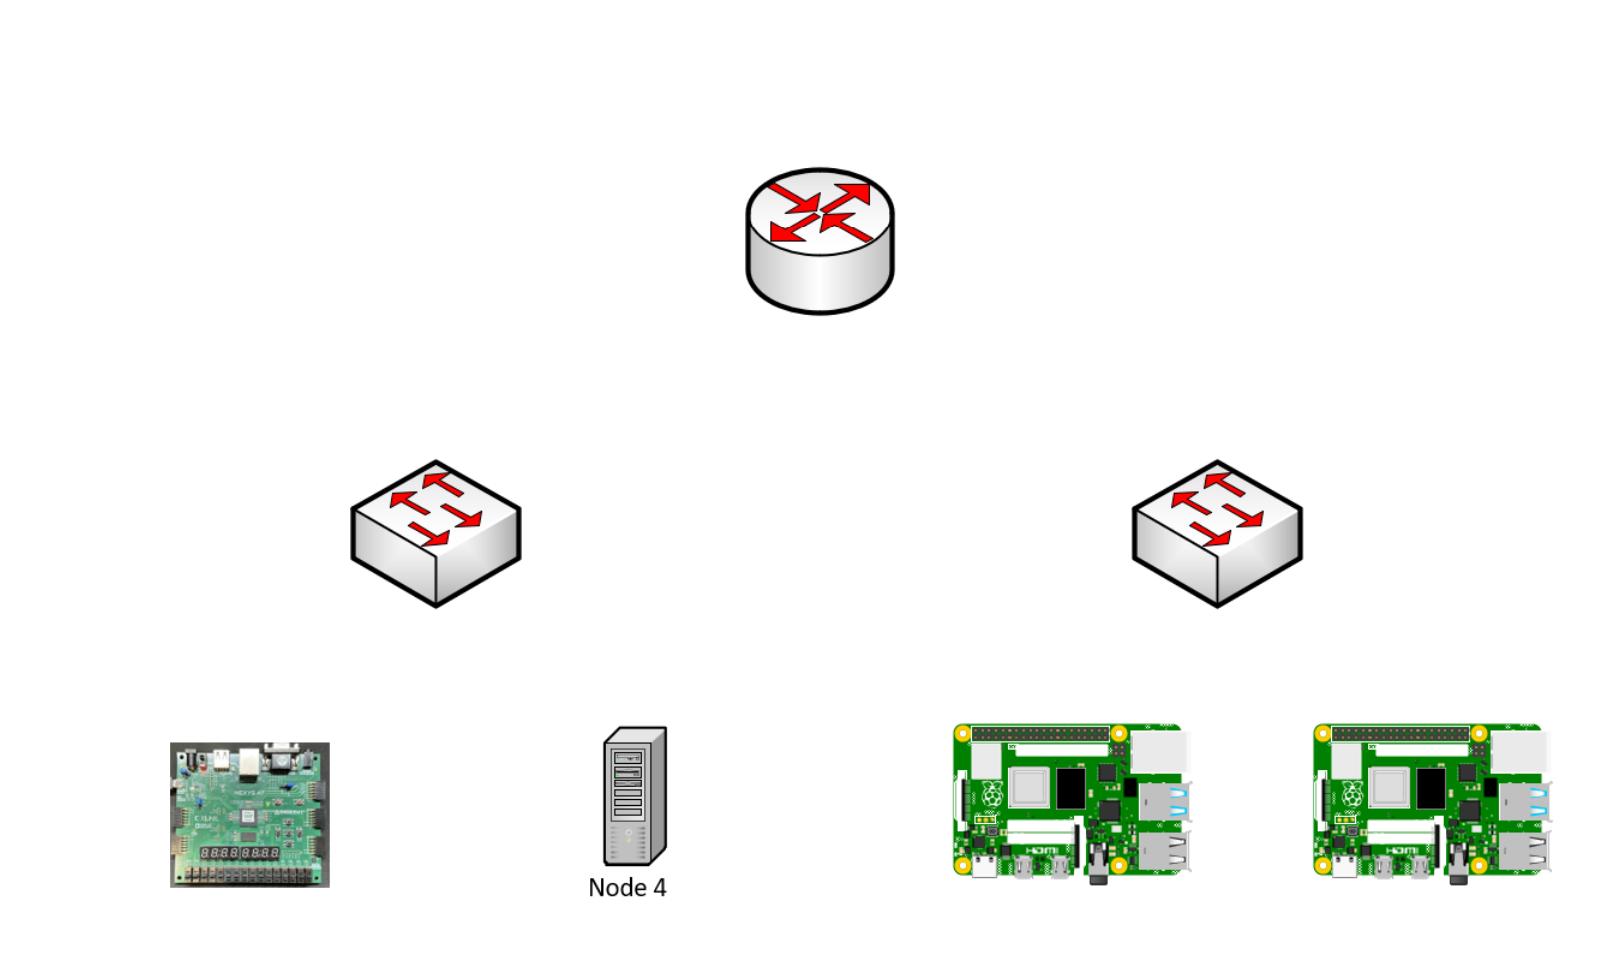
\includegraphics[width=1\textwidth]{Images/NetworkArchitecture.png}
    \caption[Network architecture for firewall tests]{Network architecture for firewall tests.}
    \label{fig:network_layout_test}
\end{figure}


The rules shown in table \ref{tab:firewall_testing_config} shows the rules that were loaded on the packet filter.  While these test cases is only a subset of the total coverage, a mix of different combinations of ports, protocols and IP addresses were chosen. More specifically the rules were chosen to test the following cases:

\begin{itemize}
    \item All devices can access the device in some way (eg, over ICMP),
    \item All machines could access at least two services,
    \item Identical ports over different protocols can be filtered (eg, port 1337 over TCP and UDP),
    \item Ports can be blocked on a device even though the device can access other services with the same protocol,
    \item The wildcard operator works in each field, and
    \item Any port that is not explicitly allowed is blocked.
\end{itemize}

By default, as the packet filter is a default-deny, any packet that doesn't fit these constraints is blocked and can be verified in the tests summarised in \ref{tab:firewall_test_cases}.


\begin{table}[h!]
    \centering
    \caption{Firewall configuration for testing}
    \label{tab:firewall_testing_config}
    \begin{tabular}{ccccc}
        \toprule
        Source IP & Destination IP & Source Port & Destination Port & Protocol \\
        \midrule
        any       & 10.20.1.34      & n/a         & n/a              & ICMP     \\
        10.0.0.5  & 10.20.1.34      & any         & any              & UDP      \\
        10.0.0.5  & 10.20.1.34      & any         & 80               & TCP      \\
        10.0.0.93 & 10.20.1.34      & any         & 1337             & TCP      \\
        10.0.0.93 & 10.20.1.34      & any         & 9999             & UDP      \\
        10.20.1.10& 10.20.1.34      & any         & 1337             & any      \\
        10.20.1.10& 10.20.1.34      & any         & any              & UDP      \\
        10.20.1.11& 10.20.1.34      & any         & 9999             & UDP      \\
        \bottomrule
    \end{tabular}
    
\end{table}

Typically, firewalls have a second interface that connects to a local network, allowing packets from multiple IP addresses to be processed and forwarded on. However, in this setup, a single device is behind the firewall, requiring the \textit{destination IP's} to be the same (the NEORV32's IP address, 10.20.1.34). 

Additionally, the \textit{source port} was configured to allow any source port through. This is important due to the client arbitrarily choosing the source port at random. Therefore, a wildcard was used as this makes the source port impossible to predict. It's worth noting that some niche programs operate with predicable ports, though none of the programs used in this test were of this nature.


\subsection{Test results}

A summary of the results can be seen in table \ref{tab:firewall_test_cases} which show the firewall blocking and allowing the respective packets correctly.

\begin{table}[h]
    \centering
    \caption{Summary of packets including expected and actual outcomes}
    \label{tab:firewall_test_cases}
    \begin{tabular}{m{2.25cm}m{2cm}m{1.5cm}m{2cm}m{2cm}m{2cm}m{2cm}}
        \toprule
        Device & Dest. IP & Protocol & Src. Port & Dest. Port & Expected Outcome & Actual Outcome \\
        \midrule
        \parbox[c]{2.25cm}{\centering Node1\\\textcolor{gray}{(10.20.1.10)} \vspace*{14pt}} & 10.20.1.34 & TCP & Any & 1337 & Allow & Allowed \\
        \parbox[c]{2.25cm}{\centering Node2\\\textcolor{gray}{(10.20.1.11)} \vspace*{14pt}} & 10.20.1.34 & ICMP & - & - & Allow & Allowed \\
        \parbox[c]{2.25cm}{\centering Node3\\\textcolor{gray}{(10.0.0.5)} \vspace*{14pt}} & 10.20.1.34 & UDP & Any & 9999 & Allow & Allowed \\
        \parbox[c]{2.25cm}{\centering Node4\\\textcolor{gray}{(10.0.0.93)} \vspace*{14pt}} & 10.20.1.34 & TCP & Any & 1337 & Allow & Allowed \\
        \parbox[c]{2.25cm}{\centering Node1\\\textcolor{gray}{(10.20.1.10)} \vspace*{14pt}} & 10.20.1.34 & UDP & Any & 1337 & Allow & Allowed \\
        \parbox[c]{2.25cm}{\centering Node3\\\textcolor{gray}{(10.0.0.5)} \vspace*{14pt}} & 10.20.1.34 & TCP & Any & 80 & Allow & Allowed \\
        \parbox[c]{2.25cm}{\centering Node3\\\textcolor{gray}{(10.0.0.5)} \vspace*{14pt}} & 10.20.1.34 & TCP & Any & 1337 & Deny & Denied \\
        \parbox[c]{2.25cm}{\centering Node2\\\textcolor{gray}{(10.20.1.11)} \vspace*{14pt}} & 10.20.1.34 & TCP & Any & 1337 & Deny & Denied \\
        \parbox[c]{2.25cm}{\centering Node4\\\textcolor{gray}{(10.0.0.93)} \vspace*{14pt}} & 10.20.1.34 & UDP & Any & 1337 & Deny & Denied \\
        \parbox[c]{2.25cm}{\centering Node4\\\textcolor{gray}{(10.0.0.93)} \vspace*{14pt}} & 10.20.1.34 & TCP & Any & 80 & Deny & Denied \\
        \bottomrule
    \end{tabular}
    
\end{table}


The detailed output from the script on each host is available in appendix \ref{app:testing_pf}. While these tests don't formally prove the firewall is correctly working, they do provide substantial evidence of the design's correctness. It's important to note that additional rigorous testing, which wasn't formally documented, was conducted throughout the development of the design. Such an example test case involves spamming ping packets from one host while sending valid packets from another. 

These results stipulate the devices suitability for use in a real world environment. The filter exhibits capacity to filter out the significant majority of unwanted packets, making it ideal for low security applications. However, formal verification and meticulous testing is imperative to suitability for high-security applications. With the absence of these in the above tests, the design would necessitate further validation to be deployed in high security environments. 


















\section{Comparison to preexisting solutions}

To ensure the effectiveness of the designed hardware, some comparisons to preexisting solutions have been made. Three other devices that featured \textit{Fast Ethernet} (100Mbit/s) connectivity were compared. These devices were the WIZ5500 Pico \footnote[1]{See: https://www.wiznet.io/product-item/w5500-evb-pico/}, Nucloe-F767ZI \footnote[2]{See: https://www.st.com/en/evaluation-tools/nucleo-f767zi.html} and MilkV-Duo \footnote[3]{See: https://milkv.io/duo}. The WIZ5500 pico board uses a \textit{Raspberry Pi RP2040} as the MCU at 133Mhz, while it uses the \textit{WIZ5500} IC for handling the Ethernet traffic. The WIZ5500 additionally handles layers 1 to 4 onboard and is interfaced over SPI. The Nucleo-F767ZI (referred to as just F767ZI) is powered by the \textit{STM32F767} MCU and features an onboard \textit{LAN8742A} PHY chip onboard. Like the Nexys board, it is also connected over an RMII interface, making it a logical comparison to the Nexys A7. The STM32 has hardware support for the RMII interface. Unlike the Nexys A7, it utilised the LwIP network stack instead of FreeRTOS-Plus-TCP. Finally, the \textit{MilkV-Duo} is the most recent RISC-V based board which features the 64-bit\textit{CVITEK CV1800B} processor. The CV1800B operates at a 1Ghz, includes 64MB of RAM and provides the MAC and PHY inside the chip itself.

\subsection{Network latency tests}


A small UDP ping program was made on the NEORV32 to receive a UDP packet on port 9999 and reply to the client to test the round trip time (RTT). This test also had the benefit of quantitatively determining the software overhead on the platform. The round trip time was then averaged over 1,000 transactions and has been presented in figure \ref{fig:avg_udp_rtt}. To determine the amount of software overhead the TCP/IP stack had on the RTT, two packets of different payloads was tested. This is because the time difference in hardware between the packet size is in the order of nanoseconds, whereas the software processing time is several orders of magnitude larger due to moving more data around and processing it. The two UDP payload sizes were 8 bytes and 256 bytes.


\begin{figure}[ht]
    \centering
    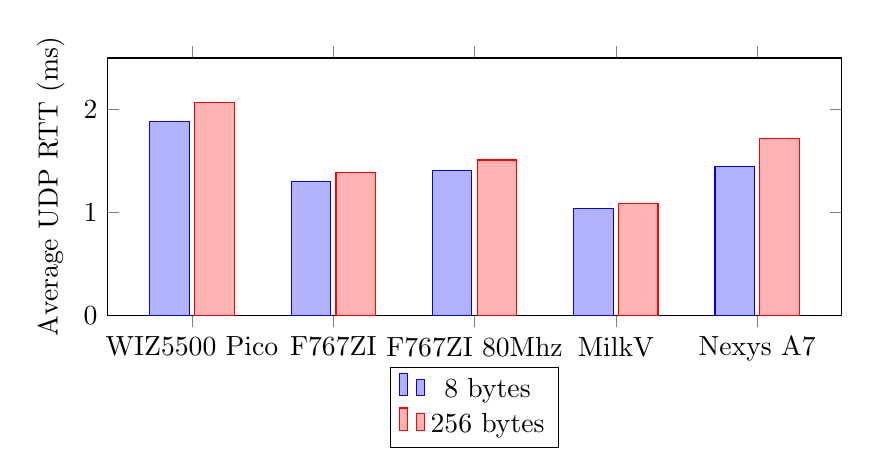
\begin{tikzpicture}
    \begin{axis}[
        ybar,
        symbolic x coords={WIZ5500 Pico, F767ZI, F767ZI 80Mhz, MilkV, Nexys A7},
        xtick=data,
        ylabel={Average UDP RTT (ms)},
        legend style={at={(0.5,-0.2)},anchor=north},
        enlarge x limits=0.15,
        ymin=0,
        ymax=2.5,
        width=0.9\textwidth,
        height=0.4\textwidth,
        bar width=0.5cm
    ]
    \addplot coordinates {
        (WIZ5500 Pico,1.88)
        (F767ZI 80Mhz,1.41)
        (F767ZI,1.30)
        (Nexys A7,1.45)
        (MilkV,1.04)
    };
    \addplot coordinates {
        (WIZ5500 Pico,2.07)
        (F767ZI 80Mhz,1.51)
        (F767ZI,1.39)
        (Nexys A7,1.72)
        (MilkV,1.09)
    };
    \legend{8 bytes,256 bytes}
    \end{axis}
    \end{tikzpicture}
    \caption{Average UDP RTT for different devices and payload sizes.}
    \label{fig:avg_udp_rtt}
    \end{figure}
    
A table of the results can be found in appendix \ref{app:udp_ping_measurements}. Testing on the Nexys A7 observed a larger difference compared to the competing products. This indicates that the software overhead on the Nexys A7 is larger. The difference in delay at the hardware level can be calculated by knowing the number of bits and the clock frequency. Fast Ethernet has a throughput of 100Mbit/s, which when sending 248 bytes results in a delay of $\frac{248 \times 8}{100 \times 10^6}=19.84\mu s$. This is likely due to the FreeRTOS-Plus-TCP stack using more computations per packet than LwIP on the F767ZI. The MilkV not only runs linux, it operates at 12.5 times the frequency, 1Ghz.

This test results indicate that the device is relatively comparable to preexisting solutions in terms of networking latency. To further compare the network performance, network throughput tests were conducted. 


\subsection{Network throughput tests}
In this section, only the F767ZI, MilkV Duo and Nexys A7 were tested. The WIZ5500 Pico was not tested as no direct support for Iperf 3 was available. Iperf 3 was used to test the bandwidth of the network between two devices. The client device was a desktop connected at gigabit speeds to the network. Iperf 3 was chosen for it's a universally accepted throughput measuring tool and that both FreeRTOS and LwIP had Iperf 3 server implementations. Table \ref{tab:bitrate_tests} summaries the bitrates of the tested devices.


\begin{table}[h]
    \centering
    \caption{Bitrate of various embedded devices}
    \label{tab:bitrate_tests}
    \begin{tabular}{P{3.5cm} P{3.5cm}}
        \toprule
        Device & Bitrate \\
        \midrule

        Nexys A7 & 1.32Mbits/s \\
        F767ZI & 7.11Mbits/s \\
        MilkV & 92.4Mbits/s \\
        \bottomrule
    \end{tabular}
    
\end{table}

It came at no surprise when the MilkV Duo with it's 1Ghz processor saturated the 100Mbits/s \textit{Fast Ethernet} interface. This test is consistent the idea that the software on the Nexys A7 is the bottleneck as alluded to in the latency tests. It is also of the belief that the FreeRTOS task priorities and interrupts on the device are not optimal which is also decreasing the performance. This was evident when changing the tick frequency in FreeRTOS from  500Hz to 1000Hz as it gave more time for the packet to be processed before switching tasks. This resulted in a 41.8\% drop in performance. The F767ZI was able to achieve a higher throughput than the Nexys A7 which is likely due to using LwIP over FreeRTOS-Plus-TCP and having more optimised drivers that handle interrupts and better task scheduling.

While the Nexys A7 provides comparable performance in the UDP ping tests, the throughput is lacking, but can be improved with optimisations in the firmware of the device. However, in having a hardware firewall, the design in this thesis has an advantage in security, which is discussed in the next section.



\subsection{Security analysis}

Only the Nexys A7 designed in this thesis employed a hardware packet filter. The other devices required a software based packet filter. The issue with software based firewalls in embedded systems is that they may be susceptible to power-glitch attacks. Power-glitch attacks are a common vulnerability in embedded systems which consists of switching off and on the power very rapidly at a critical point in the code to essentially bypass a certain instruction. While this is highly unlikely and often hard to implement, it is an advantage nonetheless for the hardware firewall.  

As the packet filter is designed in hardware and is directly reading the bits from the PHY and doesn't operate in the same way as a software implementation, the hardware packet classifier in this design should not susceptible to power-glitch attacks. Formal testing of this however was not part of the scope of this thesis. Another benefit of the design created in this thesis is the latency properties, which is discussed in the next section. 



\subsection{Firewall latency}

To measure the latency of the software firewalls accurately, a GPIO pin was configured to toggle when the packet first enters the packet filter and then again after it has been filtered. It is assumed that the latency of setting the pin high cancels out with the latency of setting the pin low and that it simply results in a phase shift and does not introduce any additional delay between the start and end. 

A software based implementation of the firewall was created on the Nucleo-F767ZI board with eight rules to make for a fair comparison as the FPGA design is limited to eight rules. Using an oscilloscope to measure the time, the measured classification delay depended on the number of rules and where a valid rule would be matched, if at all, at the start or end of the sequence. 

As a best case, the time was found to be $3.14\mu s$ (figure \ref{fig:sw_pf_best_case}) while an average-to-bad case was $10.76\mu s$ (figure \ref{fig:sw_pf_bad_case}).



\begin{figure}[h]
    \centering
    \begin{subfigure}[b]{0.45\textwidth} % Adjust the width to your needs
        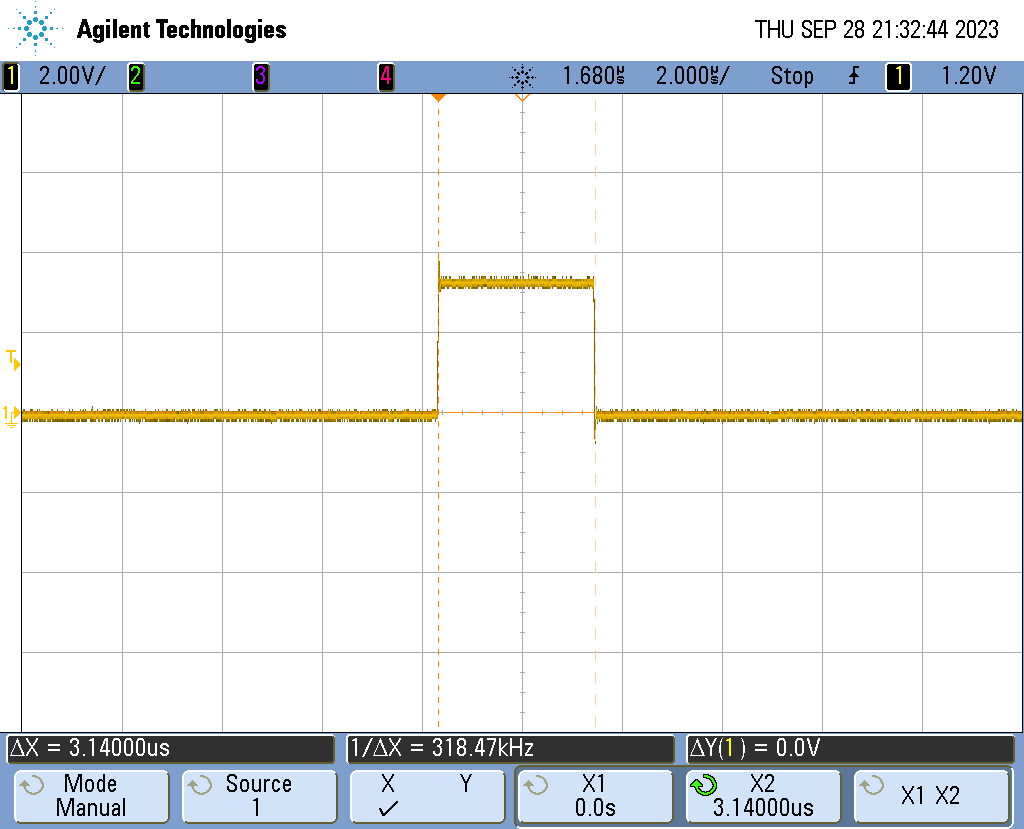
\includegraphics[width=\textwidth]{Images/sw_pf_best_case.png}
        \caption{Best case scenario}
        \label{fig:sw_pf_best_case}
    \end{subfigure}
    \hfill % this will add a small space between the two images
    \begin{subfigure}[b]{0.45\textwidth} % Adjust the width to your needs
        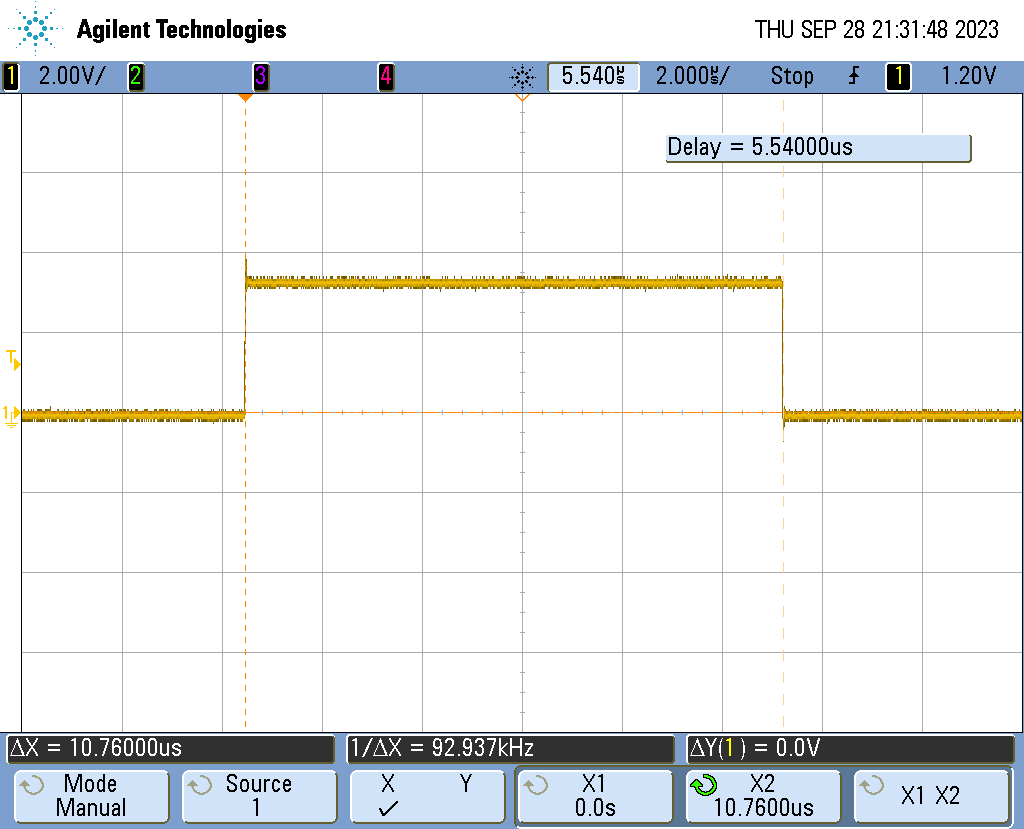
\includegraphics[width=\textwidth]{Images/sw_pf_bad_case.png}
        \caption{Average case}
        \label{fig:sw_pf_bad_case}
    \end{subfigure}
    \caption{Software packet classifier timings}
    \label{fig:sw_pf_timings}
\end{figure}

The lower delay in the ideal software case is due to the small number of rules needed to be considered reducing the number of comparisons needed to be made. In practice, it is expected that the first rule is not always matched, and hence the average case should be used for an amortised latency. Importantly these delays unlike the FPGA one, do impact throughput as the processor is limited to filtering the packets and not doing other things like receiving another packet. In a low bandwidth environment, there is little benefit other than security over a hardware firewall in an embedded system.However, if latency is critical, like it is in real time robotic control systems and bandwidth is high or even if the highest security is needed such as in secure access control systems, a hardware firewall provides a better alternative to a software implementation. Another difference between hardware and software is efficiency of the design, which will be detailed in the next section. 




\subsection{Power consumed between boards}

No measurable difference in current consumption was observed when using the packet filter in hardware over it being disabled. This is likely due to the measurment equiptment not featuring a high enough resolution. However, when implementing a software firewall, a relative current increase of 1mA was observed which is due to running more comparisons per loop. 

The remainder of this section compares the absolute current measurements recorded across the devices which can be seen in figure \ref{fig:power_comparison}. In this figure, four measurements were made, Idle, Busy, No Ethernet and Clean state. The Idle is just the design loaded, but idling and not receiving any packets. Busy is the measurement when the device is receiving packets and processing them. This is typically lower due to the flashing status LED providing more of an impact than the additional power consumed by the hardware. No Ethernet is the measurement when the Ethernet cable is unplugged and the device is idling. This is an important measurement as the PHY chips tend to implement a low power sleep state when no Ethernet cable is connected. Clean state is the measurement when the device is idling and with no design loaded. This is effectively the quiescent current consumed by the device. 


\begin{figure}[ht]
    \centering
    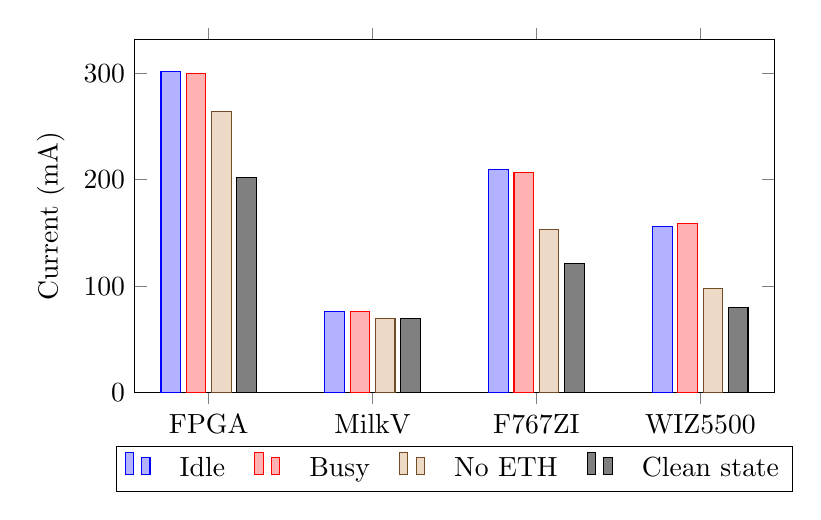
\begin{tikzpicture}
        \begin{axis}[
            ybar,
            bar width=0.25cm,
            width=0.8\textwidth,
            height=0.5\textwidth,
            enlarge x limits=0.15, % Adjusted value to make the bars closer
            ylabel={Current (mA)},
            symbolic x coords={FPGA, MilkV, F767ZI, WIZ5500},
            xtick=data,
            legend style={
                at={(0.5,-0.15)},
                anchor=north,
                legend columns=-1,
                legend cell align=left,
                legend image post style={scale=1}, % Adjust this value for spacing
                column sep=0.3cm % Adjust the space between each legend entry
            },
            legend cell align=left,
            ymin=0,
        ]
        \addplot coordinates {
            (FPGA, 301.4)
            (MilkV, 76.27)
            (F767ZI, 209.25)
            (WIZ5500, 155.88)
        };
        \addlegendentry{Idle}
        
        \addplot coordinates {
            (FPGA, 300.13)
            (MilkV, 76.53)
            (F767ZI, 206.9)
            (WIZ5500, 158.67)
        };
        \addlegendentry{Busy}
    
        \addplot coordinates {
            (FPGA, 264)
            (MilkV, 69.23)
            (F767ZI, 153.46)
            (WIZ5500, 97.9)
        };
        \addlegendentry{No ETH}

        % New data for "Complete Idle"
        \addplot coordinates {
            (FPGA, 202.13)
            (MilkV, 69.23)
            (F767ZI, 121.31)
            (WIZ5500, 80.35)
        };
        \addlegendentry{Clean state}

        \end{axis}
    \end{tikzpicture}
    \caption{Comparison of Idle, Busy, and No eth currents for devices}
    \label{fig:power_comparison}
    \end{figure}
    


In Appendix \ref{app:current_measurements} figure \ref{tab:power_consumption} shows the same data in table form presenting numerical values.

From figure \ref{fig:power_comparison}, the difference between the clean state and the busy states can be learned. The Nexys A7 had the largest difference at 99.27mA, compared to the 87.94mA difference witnessed in the F767ZI board. What must be taken into consideration is that the measurement for the Nexys A7 is without the hardware design (both Ethernet MAC, packet filter and RISC-V core) applied. Another reading of 283.75mA was observed when the design and hardware had been loaded (no firmware). What this means is that even though the Nexys A7 has the highest quiescent current amoungst the devices, it still has the larger design current for the project itself. Power optimisations would be needed to be made in both the Ethernet and RISC-V core to reduce this current to perform better than the preexisting solution. However, this was not a focus of this thesis.

As it stands, this result indicates that the Nexys A7 board is not ideal to be used in a low power environment due to its large quiescent current. The purpose of the Nexys A7 board isn't to be power efficient, but rather be used as a platform for development. In a production environment, the board design would not have unused parts and may also feature more power efficient components or FPGAs. This is not the scope of this thesis, but is an important consideration for future work.

A byproduct of current draw is heat output. By using a thermal camera, one can learn where the majority of the power is being drawn and as such is discussed in the next section.




\subsection{Thermal analysis}

A Flir One thermal camera was used to record the temperatures periodically with a summary of results presented in table \ref{tab:temperature_comparison}. Throughout the test, an ambient room temperature of $24.8\degree C$ was maintained. Measurements were made after 5, 10, 30, 60 and 120 minutes to track how the PCB board impacted the thermal properties of the chips. This is important due to the larger PCBs having a larger thermal mass, skewing the results. A table of results can be found in appendix \ref{app:thermal_measurements}. No major differences were observed in the thermal images after 60 minutes, hence results halted at the 120-minute mark.

\begin{table}[h]
    \centering
    \caption{Temperature comparison of different chips during the test}
    \label{tab:temperature_comparison}
    \begin{tabular}{P{3.5cm} P{3.5cm} P{3.5cm} }
        \toprule
        Time & Chip & Temperature ($\degree C$) \\
        \midrule
        5 min & WIZ5500 & 58.0  \\
              & FPGA & 38.0 \\
              & MilkV & 36.7 \\
              & F767ZI & 35.9 \\
        \midrule
        2 hours & WIZ5500 & 56.8 \\
                & FPGA & 40.4 \\
                & MilkV & 38.1 \\
                & F767ZI & 36.8 \\
        \bottomrule
    \end{tabular}
\end{table}

The thermal distribution on each of these boards after two hours can be seen in figure \ref{fig:thermal_2hr}. It is important to note the measurements cannot be considered as accurate, but rather should be interpreted as an indication to the hotspots and the relative temperatures of the chips to everything else on the board. Variations due to the self calibration procedure and aiming of the thermal camera to record the hottest part are expected.


\begin{figure}[h]
    \centering
    \begin{subfigure}[b]{0.45\textwidth} % Adjust the width to your needs
        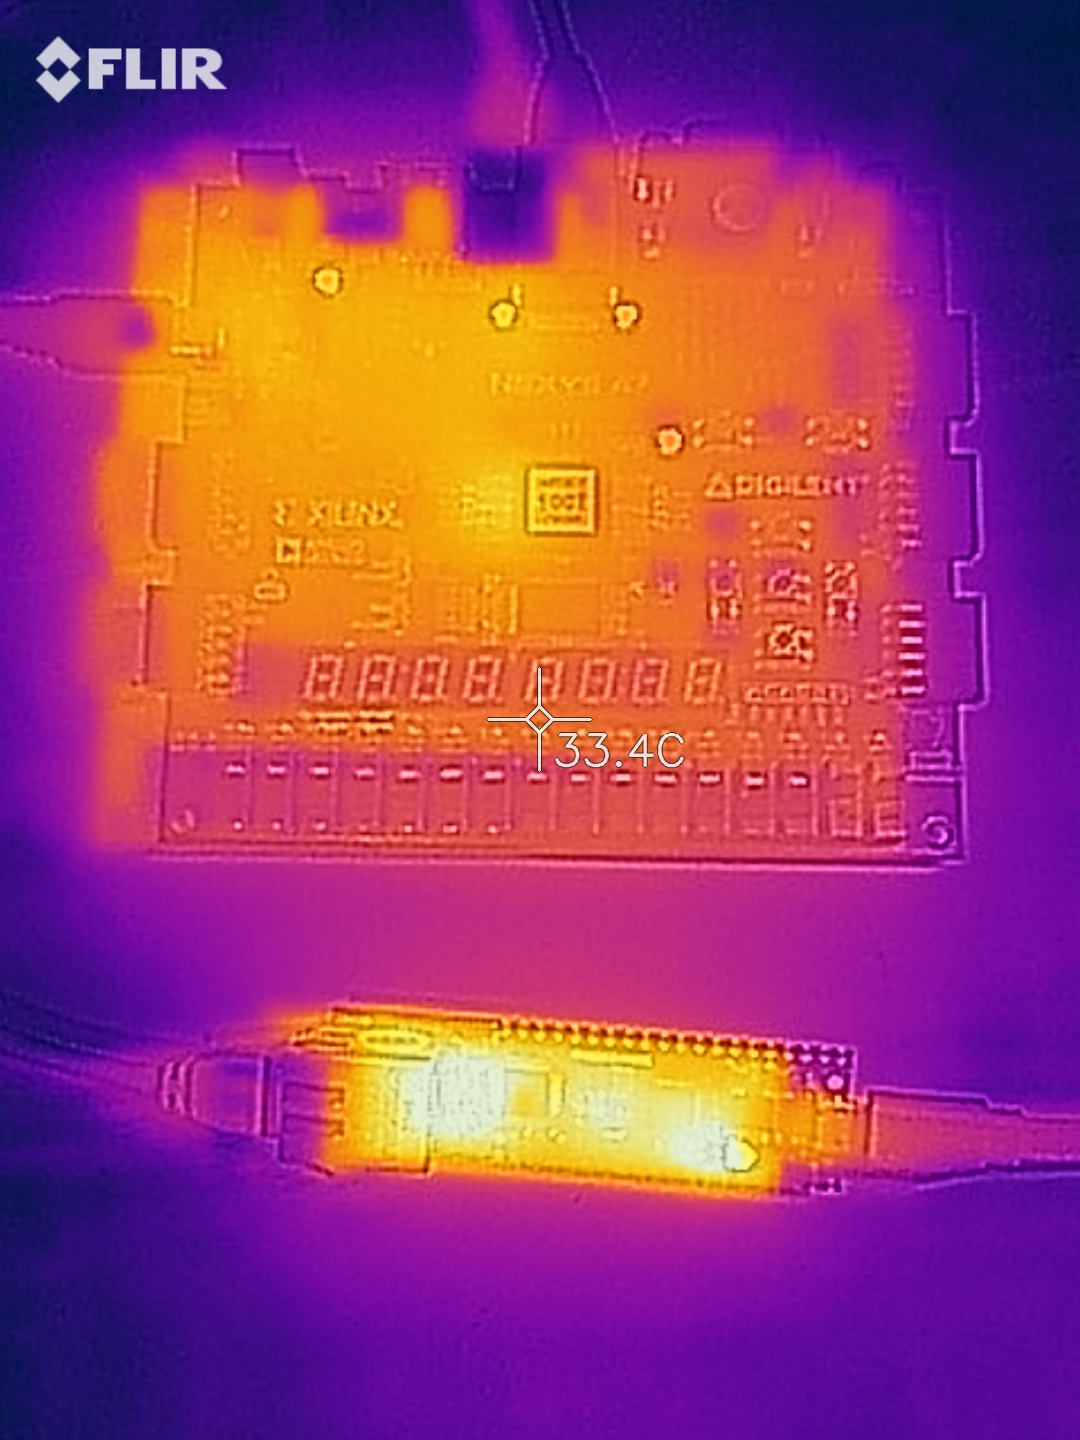
\includegraphics[width=\textwidth]{Images/flir_2hs.jpg}
        \caption{Nexys A7 (top) and WIZ5500 Pico (bottom)}
        \label{fig:thermal_2hr_fpga_pico}
    \end{subfigure}
    \hfill % this will add a small space between the two images
    \begin{subfigure}[b]{0.45\textwidth} % Adjust the width to your needs
        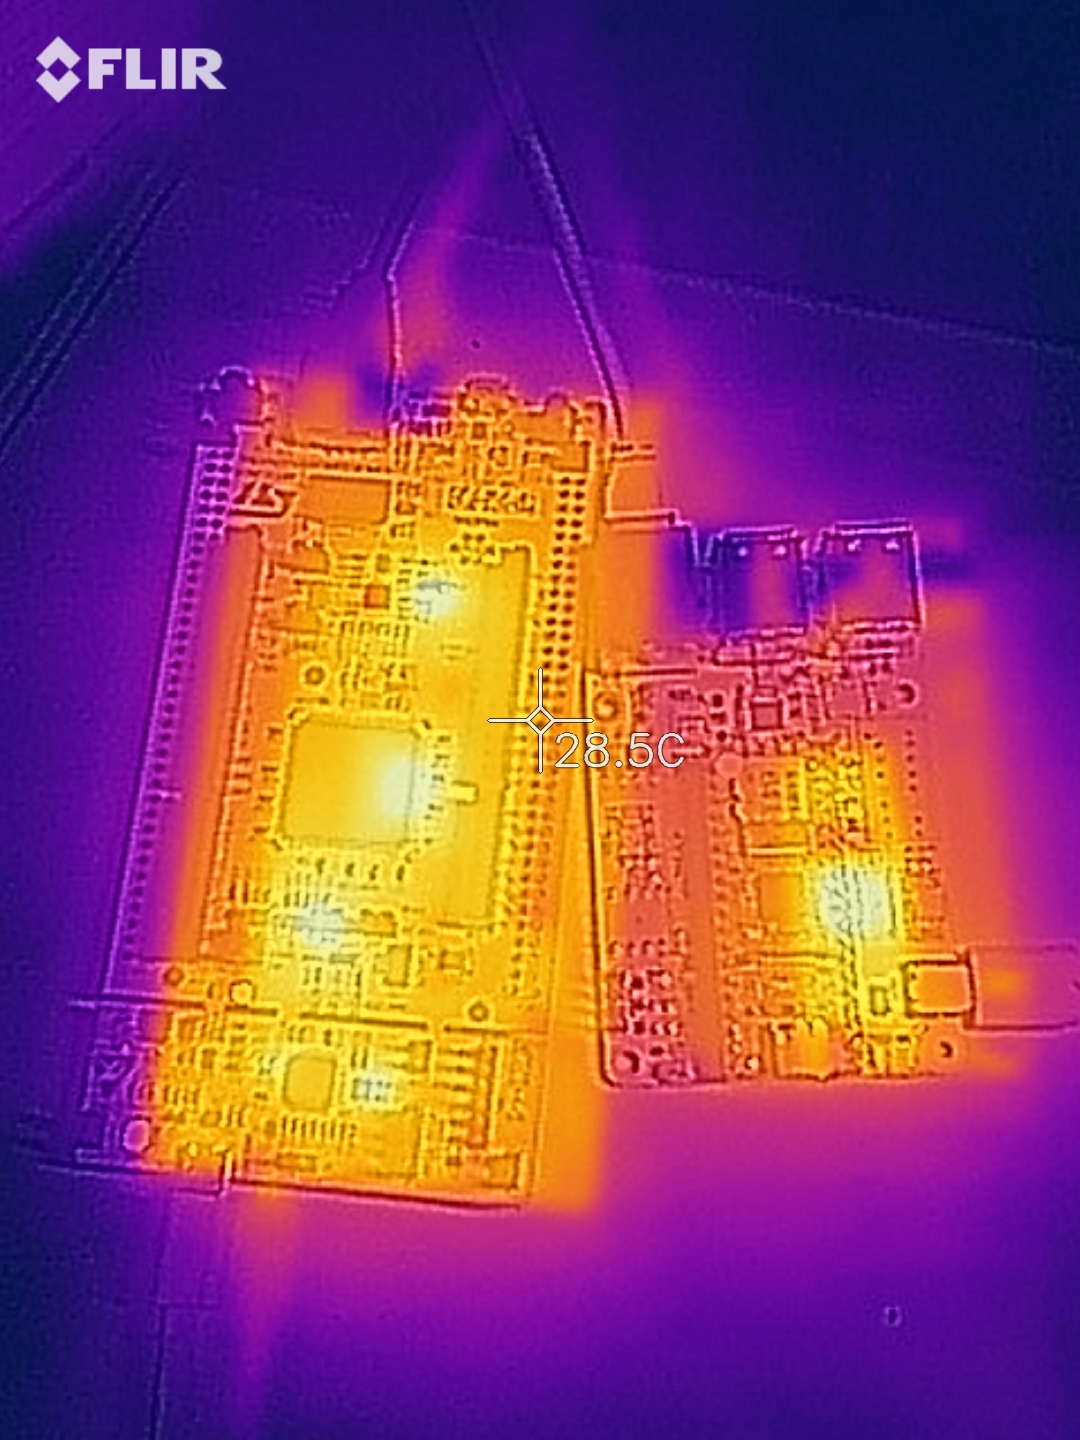
\includegraphics[width=\textwidth]{Images/flir_nucleo_milkv.jpg}
        \caption{Nucleo board (left) and MilkV Duo (right)}
        \label{fig:thermal_2hr_nucleo_milkv}
    \end{subfigure}
    \caption{Thermal images of boards under test after two hours}
    \label{fig:thermal_2hr}
\end{figure}


From the figure \ref{fig:thermal_2hr_fpga_pico}, the Nexys A7 seems to have other hotspots on the board other than the FPGA itself. This is what is likely causing the higher quiescent current in the previous section. Relatively compared to the other designs, the Nexys A7 shows minimal heat output, indicating a more efficient design. It is important to remember the physical sizes of the chips and the thermal mass behind them. 

The WIZ5500 seems to reach the hottest out of the boards tested, while the MilkV board seems to output the least amount of heat radiated. The F767ZI board records a lower temperature, but is significantly larger in chip size and PCB size. In addition, the F767ZI has an additional PHY chip which also adds to the thermal output. The MilkV in comparison only has one small chip with the MCU, MAC and PHY in the same package. These results indicate that the WIZ5500 is inefficient and may not be suitable for use in temperature sensitive environments such as recording temperature measurements in a room, wheras the MilkV or FPGA on a different board may be more suitable.

While these thermal tests don't provide a great deal of useful information, it does help support the idea that a lot of the current drawn by the Nexys A7 is not from the FPGA itself and that the device is relatively efficient. The following section delves deeper into the power consumption aspects of the design.




























\section{Power analysis}

\subsection{Theoretical analysis }

Vivado provides a post synthesis power analysis summary for the design. While these are depenant on a lot of variables, they should provide a basis as to what to expect and help with optimisation of power within the design. The design was observed to take a total of 0.487W (figure \ref{fig:post_synth_power_summary}) where 0.383W of that is dynamic and depends on the operations taking place. 

\begin{figure}[h]
    \centering
    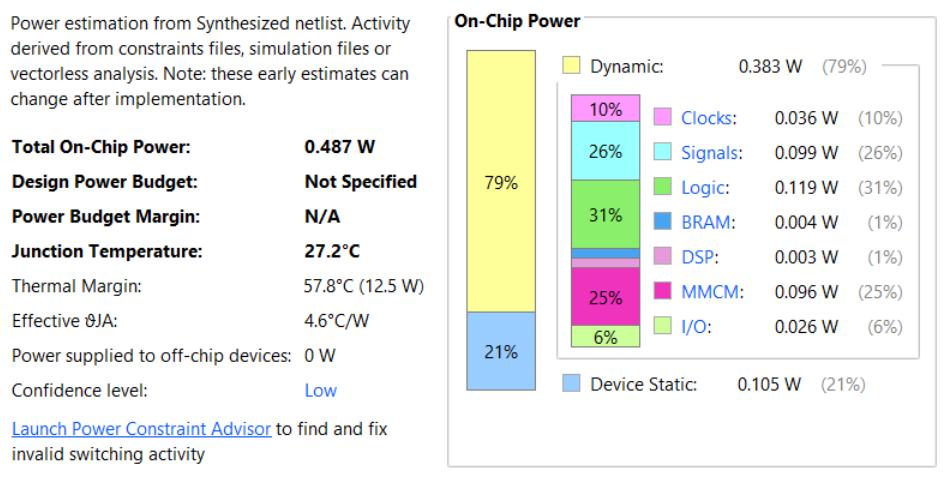
\includegraphics[width=0.75\textwidth]{Images/power_summary.png}
    \caption[Post synthesis power summary for design]{Post synthesis power summary for design.}
    \label{fig:post_synth_power_summary}
\end{figure}


Vivado further breaks down the design into the different hierarchical components shown in table \ref{tab:power_consumption}. Notably most of the power consumption in the design is a result of the RISC-V processor in the design. Notably the Ethernet hardware and packet filter consumes under 100mW. 

\begin{table}
    \centering
    \caption{Power consumption of components.}
    \begin{tabular}{lc}
        \toprule
        Name & Total (W) \\
        \midrule
        neorv32 & 0.158 \\
        clk control & 0.097 \\
        ethernet\_mac & 0.097 \\
        packet classifier & 0.002 \\
        \bottomrule
    \end{tabular}
    \label{tab:power_consumption}
\end{table}






\subsection{Measured analysis}

As the voltage would remain constant between devices (all powered over USB), only the current was measured. These results however should be taken with caution as they do not account for regulator inefficiencies and do not give a true current reading of the device, rather just an indication. 


The device for testing the current was the Nordic Semiconductor Power Profiler Kit 2 which can record at up to 100kSa/s. For the tests in this report, only a sampling rate of 10kSa/s was used as it produces less noisy results. 

As a baseline, the Nexys A7 board draws 200mA (1W at 5V) with no design applied and is due to all the additional components on the board. With the design loaded up but without the processor flashed, the board took 284.4mA. After flashing the board, the idle current reached an average of 301.84mA. Multiplying this by 5V gives us a power draw of 1.51W. To factor in the quiescent current for the other devices on the Nexys A7 and if it is assumed that the 200mA reading solely for the other components on the Nexys A7, it can be found that the design draws around 0.51W. This is rather close to what the synthesis tool calculated. 

A series of tests were then done and the currents were measured. By pinging the device every 50ms, the average current consumption was 300.72mA. Interestingly, the current consumption was cyclic similar to what is shown in figure \ref{fig:ppk_icmp_ping}. A UDP ping test was conducted and had an average current draw of 301.13mA. In both the ICMP and UDP pings, the current consumption was of similar style where the variance of the current was about 10mA. 


If the packets are now blocked by the filter, more about the design in terms of power consumption can be learned. After adding a rule in the packet filter, very little could be observed in the current consumption over the unblocked case. The same cyclic pattern in figure \ref{fig:ppk_icmp_ping} could be seen. An average of 300.92mA was been consumed by the device and is within the margin of error of the device. Figure \ref{fig:ppk_icmp_ping} shows the that the period for the current waveform is about 83ms, which is much larger than the 50ms between pings to the device. After filming the status LED on the PHY output at 240 frames per second, the period of the LED was 20 frames equivalent to $\approx 84ms$ which aligns with the current measurements. 


\begin{figure}[h]
    \centering
    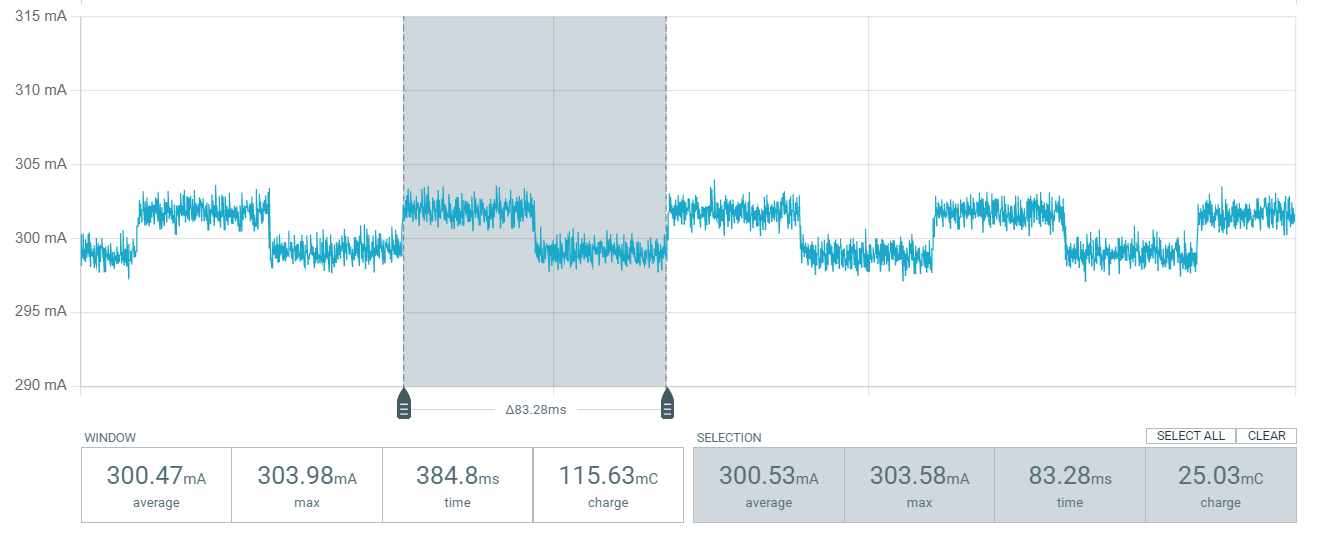
\includegraphics[width=0.9\textwidth]{Images/PPK_ping_zoom.png}
    \caption[Zoomed in current consumption for ICMP pings]{Zoomed in current consumption for ICMP pings.}
    \label{fig:ppk_icmp_ping}
\end{figure}



The next test was done when accessing the webserver. Figure \ref{fig:ppk_http_annotated} shows 5 different regions where each region is a result of a different action. The left most tests is from the inital HTTP requests to get the index page. Notably, there is 2 separate sections here, this is because the client fetches the html, css and favicon first and then requests the main (and much larger) javascript file after. The readings for each of these points is given as: average current, maximum current and time going from top to bottom. 

The second test is what happens when you click to navigate to the about page. The third event is when navigating to the config page and the 4th event is what happens when you press the 'load rules' button. The final test case is a refresh on the main page for the statistics. Notably, as the javascript (thus client) is doing the routing and page handling, future requests to get the contents of the pages are not needed, but only small API requests to update the data. Coincidentally, these first 3 requests also trigger a SD card read and explains the higher current draw. The fourth request also creates a read request to the SD card, but only needs to read a single page. The fifth request does not involve a read or write to the SD card, but rather just a simple SPI transaction takes place and consequently doesn't draw much additional power. 

\begin{figure}[h]
    \centering
    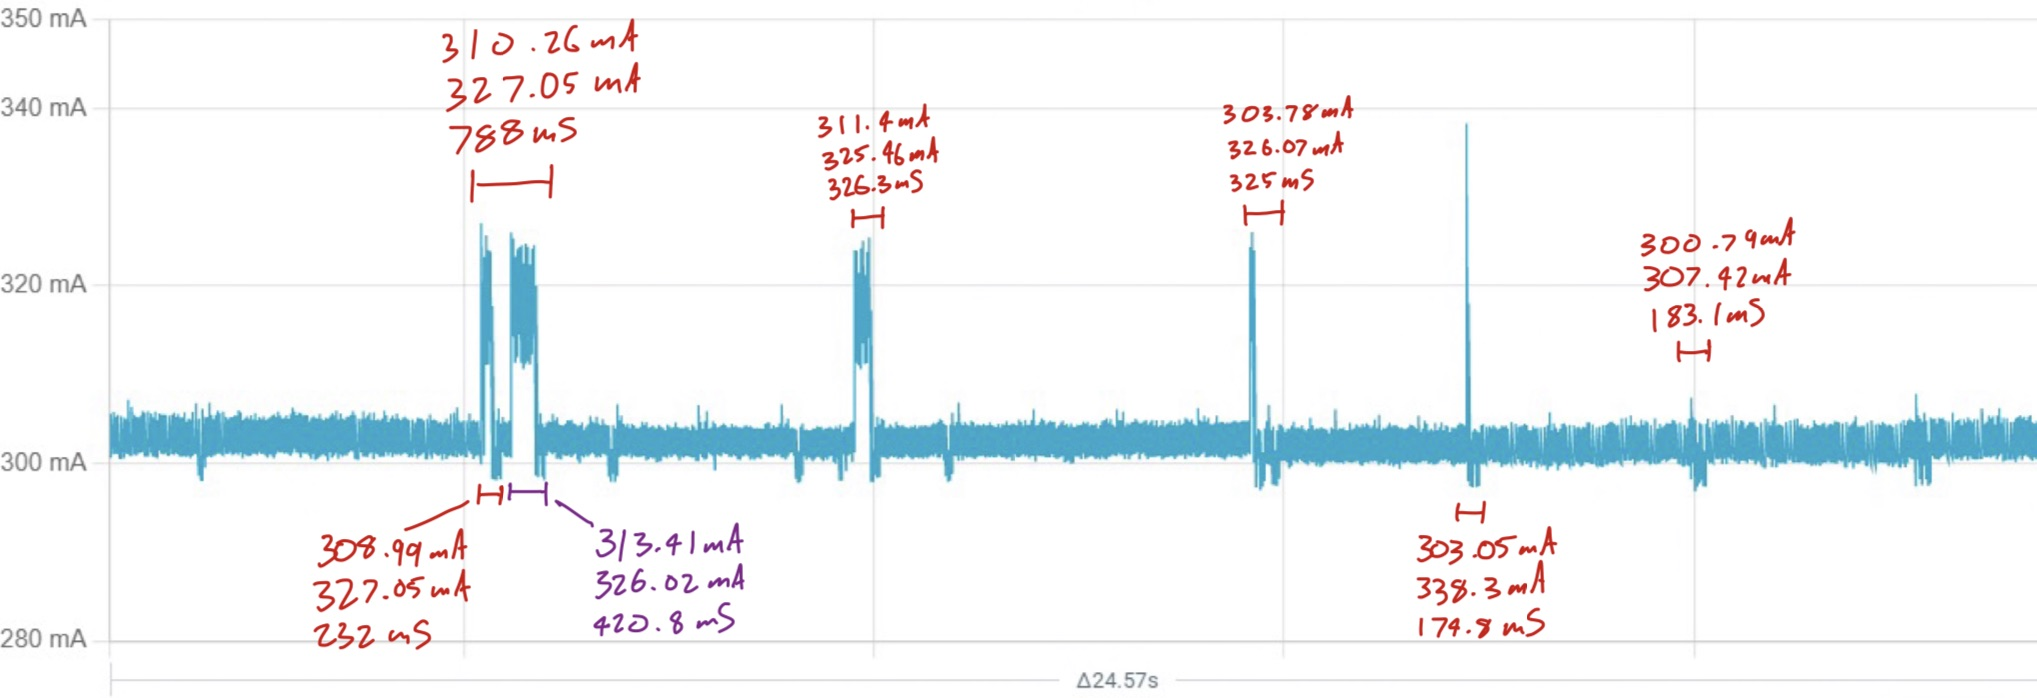
\includegraphics[width=0.9\textwidth]{Images/PPK_http_annotated.png}
    \caption[Current consumption of Nexys A7 with HTTP requests]{Current consumption of Nexys A7 with HTTP requests.}
    \label{fig:ppk_http_annotated}
\end{figure}





























\section{Modifications}
The design was changed from the 2 ethernet interfaces to a design with just a single ethernet interface. 
\subsection{Limitations}
\subsubsection{PMOD Interface}

There are 5 PMOD connectors on the development board. Initally, one of these would be used for a second Ethernet PHY, but due to bandwidth limitations of the interface, the design had to be altered. The recommended bandwidth of these ports are 25MHz while the Ethernet RMII PHY would have been using 50Mhz signals over the interface. As such, signal integrity issues arose (see figure \ref{fig:eye_diagram}) and restricted the use to just one interface - the onboard PHY. A new development board with two PHYs would be needed.

\begin{figure}[h]
    \centering
    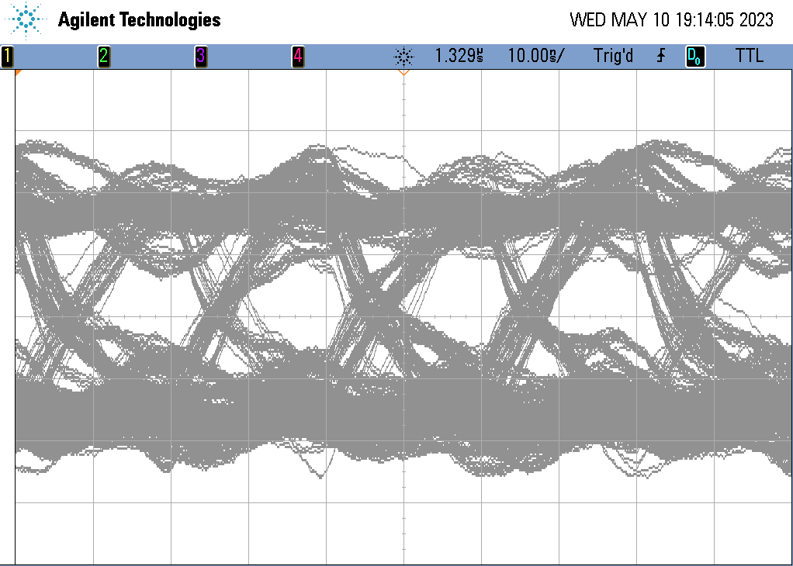
\includegraphics[width=0.65\textwidth]{Images/EyeDiagramTX.png}
    \caption[Eye diagram of TXD through PMOD interface]{Eye diagram of TXD through PMOD interface.}
    \label{fig:eye_diagram}
\end{figure}